\flashcard{
  In a tree, if node $u$ is the \textbf{parent (ancestor)} node of $v$, then $v$ is a \blank{child} (\blank{descendent}) of $u$. Two children of the same parent are \blank{siblings}.
}

\card{What is a tree?}{
  A tree $T$ is a non-empty set of nodes storing useful information in a parent-child relationship with the following properties: \\
  $T$ has a special node $r$ referred to as the root. \\ 
  Each node $v$ of $T$ different from $r$ has a parent node $u$.
}

\flashcard{
  In a tree, an external node is known as \blank{a leaf node}. It has no \blank{children}. 
}

\flashcard{
  In a tree, an internal node has one or more \blank{children}. 
}

\card{
  What do we do here?\\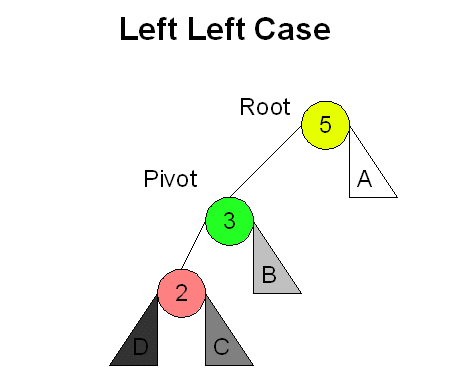
\includegraphics[height=0.8\cardheight]{images/left-left}
}{
  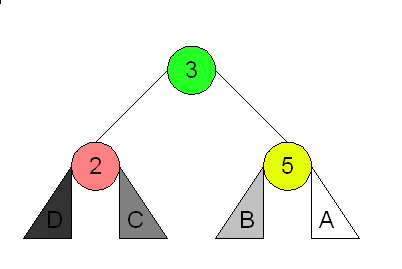
\includegraphics[height=0.8\cardheight]{images/left-left-out}
}

\card{
  What do we do here?\\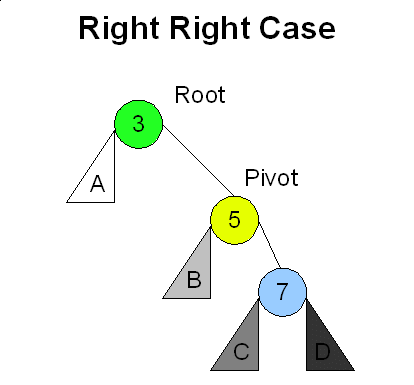
\includegraphics[height=0.8\cardheight]{images/right-right}
}{
  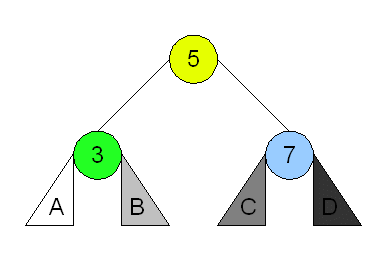
\includegraphics[height=0.8\cardheight]{images/right-right-out}
}

\card{
  What do we do here?\\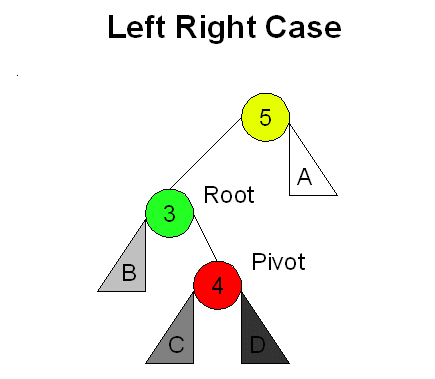
\includegraphics[height=0.8\cardheight]{images/left-right}
}{
  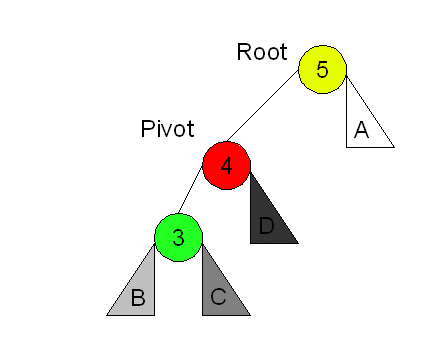
\includegraphics[height=0.8\cardheight]{images/left-right-mid}\\
  Then a left-left!
}

\card{
  What do we do here?\\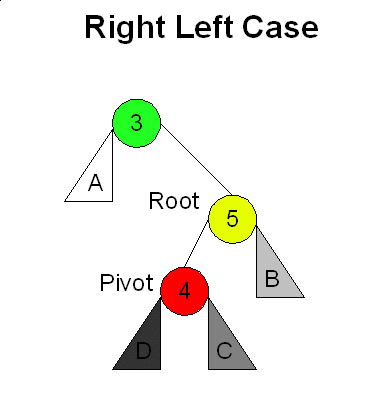
\includegraphics[height=0.8\cardheight]{images/right-left}
}{
  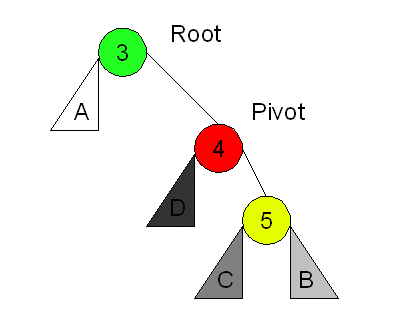
\includegraphics[height=0.8\cardheight]{images/right-left-mid}\\
  Then a right-right!
}

\card{
  What does a Depth First Search use?
}{
  A stack!
}

\card{
  What does a Breadth First Search use?
}{
  A queue!
}

\card{
  What is the running time of Dijkstra's algorithm?
}{
  $O(E + V\log(v))$
}

\card{
  What's the running time of a depth first search when the graph is an adjacency
  matrix?
}{
  $O(V^2)$ since finding neighbours takes $O(V)$ time.
}

\card{
  What's the running time of a depth first search when the graph is an adjacency
  list?
}{
  $O(V + E)$
}

\card{
  How do we insert an element into a heap?
}{
  First, you insert it at the next space in the heap (last element of current
  row, or a new row), then you keep swapping it with its parent if the parent
  is larger than it.
}

\card{
  How do we remove the smallest element from a (min) heap?
}{
  We move the last element from the heap to the first element (we can override
  the first element since we've removed it). Now we `down heap' by swapping
  the moved node with its smallest child until it is smaller than both its
  children or it has no children.
}

% Priority Queue %

\card{What is a priority queue?}{
  A \textbf{priority queue} $P$ is a container of elements with keys associated to them at the time of insertion.\\
  \begin{flushleft}
    - $insertItem(k, e)$: Inserts an element $e$ with key $k$ into $P$.
    - $removeMin()$: Returns and removes from $P$ an element with the smallest key.
  \end{flushleft}
  Two fundamental methods in a priority queue.
}

% Heap %

\card{What is a heap?}{
  A \textbf{heap} is a binary that stores a collection of keys at its internal nodes that satifies two addtional properties: \\
  A relational property that affects how the keys are stored and a structural property. \\
  It allows insertions and removals to be performed in logarithmic time.
}

\flashcard{
  A \textit{heap-based priority queue} consists of: \\
  \blank{Heap}: A complete binary tree with keys that satisfy the heap-order property.\\
  \blank{Last}: A reference to the last node in $T$.\\
  \blank{Comp}: A comparator that defines the total order relation among keys. 
}

\card{What is an \textbf{AVL Tree}?}{
  An AVL tree is another balanced binary search tree. Named after their inventors, Adelson-Velskii and Landis, they were the first dynamically balanced trees to be proposed. Like red-black trees, they are not perfectly balanced, but pairs of sub-trees differ in height by at most 1, maintaining an $O(logn)$ search time.
}

\card{What is \textbf{graph colouring}?}{
  In graph theory, graph coloring is a special case of graph labeling; a coloring of graph with $k$ colours is allocation of the colours to the nodes of the graph, such that each node has just one colour and nodes linked by an edge have different colours.
}

\flashcard{
  The minimum number of colours require to colour a graph is its \blank{chromatic number}.
}

\flashcard{
  Graph colouring is an example of an NP-complete problem. The only algorithms known for NP-complete problems are \blank{exponential}.
}

\card{Describe the difference between a \textbf{directed} and \textbf{undirected graph}. Give an example of each.}{
  An undirected graph is one where more than one edge is possible between a pair of nodes. \\
  Directed example: Trees, Utility networks. \\
  Undirected example: Graphic models, Social networks, Transport links.
}

\flashcard{
  An edge is \blank{incident} on a node if it has the node as source or target (directed) or if it links the node to another (undirected).
}

\card{Define the terms \textbf{sparse} and \textbf{dense} in the context of graphs.}{
  A graph is sparse if it has few edges, more specifically, $Edges=O(Nodes)$.\\
  It is dense if most pairs of nodes are joined by edges. More specifically, $Edges=O(Nodes^2)$
}

\card{What is a \textbf{connected component} of a graph $G$?}{
  The largest connected sub-graph (i.e. the one that cannot be expanded with additional nodes without becoming disconnected.)
}

\card{What is the Pseudo-code for Depth-first search?}{
  \begin{flushleft}
    forall nodes $u$ do $dfsnum(u)=0$ end;\\
    $i=0$; \\ 
    visit(u): \\
    \tab $i++$; \\
    \tab $dfsnum(v)=i$;\\
    \tab forall nodes $v$ adjacent to $u$: \\
    \tab \tab if $dfsnum(v)=0$ \\
    \tab \tab visit(v); \\
    forall nodes $u$: \\
    \tab if $dfsnum(u)=0$ \\ 
    \tab \tab visit(u);
  \end{flushleft}
  Depth-first search
}

\card{How do you do a \textbf{Depth-First Search}?}{
  Visit all descendants of a node, before visiting sibling nodes. Revisiting of nodes takes place through backtracking.
}

\card{How do you do a \textbf{Breadth-First Search}}{
  Visit all children of a node, then all children of those nodes.
}

\card{How do you do a priority search?}{
  Visit the root node. At each step, visit a node that has the \textbf{highest priority} amongst unvisited children of visited nodes.
}